\documentclass[english,man]{apa6}

\usepackage{amssymb,amsmath}
\usepackage{ifxetex,ifluatex}
\usepackage{fixltx2e} % provides \textsubscript
\ifnum 0\ifxetex 1\fi\ifluatex 1\fi=0 % if pdftex
  \usepackage[T1]{fontenc}
  \usepackage[utf8]{inputenc}
\else % if luatex or xelatex
  \ifxetex
    \usepackage{mathspec}
    \usepackage{xltxtra,xunicode}
  \else
    \usepackage{fontspec}
  \fi
  \defaultfontfeatures{Mapping=tex-text,Scale=MatchLowercase}
  \newcommand{\euro}{€}
\fi
% use upquote if available, for straight quotes in verbatim environments
\IfFileExists{upquote.sty}{\usepackage{upquote}}{}
% use microtype if available
\IfFileExists{microtype.sty}{\usepackage{microtype}}{}

% Table formatting
\usepackage{longtable, booktabs}
\usepackage{lscape}
% \usepackage[counterclockwise]{rotating}   % Landscape page setup for large tables
\usepackage{multirow}		% Table styling
\usepackage{tabularx}		% Control Column width
\usepackage[flushleft]{threeparttable}	% Allows for three part tables with a specified notes section
\usepackage{threeparttablex}            % Lets threeparttable work with longtable

% Create new environments so endfloat can handle them
% \newenvironment{ltable}
%   {\begin{landscape}\begin{center}\begin{threeparttable}}
%   {\end{threeparttable}\end{center}\end{landscape}}

\newenvironment{lltable}
  {\begin{landscape}\begin{center}\begin{ThreePartTable}}
  {\end{ThreePartTable}\end{center}\end{landscape}}

  \usepackage{ifthen} % Only add declarations when endfloat package is loaded
  \ifthenelse{\equal{\string man}{\string man}}{%
   \DeclareDelayedFloatFlavor{ThreePartTable}{table} % Make endfloat play with longtable
   % \DeclareDelayedFloatFlavor{ltable}{table} % Make endfloat play with lscape
   \DeclareDelayedFloatFlavor{lltable}{table} % Make endfloat play with lscape & longtable
  }{}%



% The following enables adjusting longtable caption width to table width
% Solution found at http://golatex.de/longtable-mit-caption-so-breit-wie-die-tabelle-t15767.html
\makeatletter
\newcommand\LastLTentrywidth{1em}
\newlength\longtablewidth
\setlength{\longtablewidth}{1in}
\newcommand\getlongtablewidth{%
 \begingroup
  \ifcsname LT@\roman{LT@tables}\endcsname
  \global\longtablewidth=0pt
  \renewcommand\LT@entry[2]{\global\advance\longtablewidth by ##2\relax\gdef\LastLTentrywidth{##2}}%
  \@nameuse{LT@\roman{LT@tables}}%
  \fi
\endgroup}


  \usepackage{graphicx}
  \makeatletter
  \def\maxwidth{\ifdim\Gin@nat@width>\linewidth\linewidth\else\Gin@nat@width\fi}
  \def\maxheight{\ifdim\Gin@nat@height>\textheight\textheight\else\Gin@nat@height\fi}
  \makeatother
  % Scale images if necessary, so that they will not overflow the page
  % margins by default, and it is still possible to overwrite the defaults
  % using explicit options in \includegraphics[width, height, ...]{}
  \setkeys{Gin}{width=\maxwidth,height=\maxheight,keepaspectratio}
\ifxetex
  \usepackage[setpagesize=false, % page size defined by xetex
              unicode=false, % unicode breaks when used with xetex
              xetex]{hyperref}
\else
  \usepackage[unicode=true]{hyperref}
\fi
\hypersetup{breaklinks=true,
            pdfauthor={},
            pdftitle={R you ready for some data?},
            colorlinks=true,
            citecolor=blue,
            urlcolor=blue,
            linkcolor=black,
            pdfborder={0 0 0}}
\urlstyle{same}  % don't use monospace font for urls

\setlength{\parindent}{0pt}
%\setlength{\parskip}{0pt plus 0pt minus 0pt}

\setlength{\emergencystretch}{3em}  % prevent overfull lines

\ifxetex
  \usepackage{polyglossia}
  \setmainlanguage{}
\else
  \usepackage[english]{babel}
\fi

% Manuscript styling
\captionsetup{font=singlespacing,justification=justified}
\usepackage{csquotes}
\usepackage{upgreek}

 % Line numbering
  \usepackage{lineno}
  \linenumbers


\usepackage{tikz} % Variable definition to generate author note

% fix for \tightlist problem in pandoc 1.14
\providecommand{\tightlist}{%
  \setlength{\itemsep}{0pt}\setlength{\parskip}{0pt}}

% Essential manuscript parts
  \title{R you ready for some data?}

  \shorttitle{R you ready}


  \author{Rick O. Gilmore\textsuperscript{1,2}, James LeBreton\textsuperscript{1}, \& Michael Hallquist\textsuperscript{1}}

  \def\affdep{{"", "", ""}}%
  \def\affcity{{"", "", ""}}%

  \affiliation{
    \vspace{0.5cm}
          \textsuperscript{1} The Pennsylvania State University\\
          \textsuperscript{2} Databrary.org  }

  \authornote{
    \newcounter{author}
    The authors are with the Department of Psychology at The Pennsylvania
    State University. The authors acknowledge support from the Department of
    Psychology and the Social, Life, \& Engineering Sciences Imaging Center
    (SLEIC).

                      Correspondence concerning this article should be addressed to Rick O. Gilmore, Department of Psychology, The Pennsylvania State University, University
Park, PA 16802 USA. E-mail: \href{mailto:rogilmore@psu.edu}{\nolinkurl{rogilmore@psu.edu}}
                                    }


  \abstract{Want to write a paper using R Markdown? Keep reading to see how.}
  \keywords{APA, R Markdown \\

    \indent Word count: Not that many.
  }





\usepackage{amsthm}
\newtheorem{theorem}{Theorem}
\newtheorem{lemma}{Lemma}
\theoremstyle{definition}
\newtheorem{definition}{Definition}
\newtheorem{corollary}{Corollary}
\newtheorem{proposition}{Proposition}
\theoremstyle{definition}
\newtheorem{example}{Example}
\theoremstyle{remark}
\newtheorem*{remark}{Remark}
\begin{document}

\maketitle

\setcounter{secnumdepth}{0}



It is possible to write an entire APA-formatted article in R Markdown.
This very brief paper shows how it might be done. As illustration, we
use the data from a brief, informal survey of participants in the
inaugural R Bootcamp at Penn State. We predicted that higher levels of
enthusiasm for \enquote{Game of Thrones} would be reported by
respondents with \emph{lower} reported hours/day of preferred sleep, at
least among younger respondents.

\section{Methods}\label{methods}

Consistent with open and transparent science practices, we report how we
determined our sample size, all data exclusions (if any), all
manipulations, and all measures in the study (Simmons, Nelson, \&
Simonsohn, 2011).

\subsection{Participants}\label{participants}

We asked participants in an optional \enquote{R Bootcamp} held at the
Pennsylvania State University Department of Psychology to complete an
anonymous survey using a Google Form. We asked participants to report
their age in years. A total of 50 respondents answered the survey with a
reported age of {[}22-55{]} years.

\subsection{Material}\label{material}

The survey can be found at this URL:
\url{https://docs.google.com/forms/d/1l5OX8PcN_lfVn3ykr_PtHCzhRbWzMbxhqtgILD45zRg/edit}.
There were five questions asked:

\begin{enumerate}
\def\labelenumi{\arabic{enumi}.}
\tightlist
\item
  Your current level of experience/expertise with R
\item
  Your enthusiasm for Game of Thrones {[}1..10 scale{]}
\item
  Age in years
\item
  Preferred number of hours spent sleeping/day
\item
  Favorite day of the week?
\item
  Are your data tidy?
\end{enumerate}

\subsection{Procedure}\label{procedure}

We emailed a link to the survey to the list of participants. We also
include a link to the survey on the web page containing the course
schedule
(\url{https://psu-psychology.github.io/r-bootcamp/schedule.html}). We
encouraged participants to complete the survey after the first day's
material.

\subsection{Data analysis}\label{data-analysis}

We used R (3.4.1, R Core Team, 2017) and the R-packages \emph{bindrcpp}
(0.2, Müller, 2016), \emph{dplyr} (0.5.0, Wickham \& Francois, 2016),
\emph{Formula} (1.2.1, Zeileis \& Croissant, 2010), \emph{ggplot2}
(2.2.1, Wickham, 2009), \emph{googlesheets} (0.2.2, Bryan \& Zhao,
2017), \emph{Hmisc} (4.0.3, Harrell Jr, Charles Dupont, \& others.,
2017), \emph{lattice} (0.20.35, Sarkar, 2008), \emph{papaja}
(0.1.0.9492, Aust \& Barth, 2017), \emph{purrr} (0.2.2.2, Henry \&
Wickham, 2017), \emph{readr} (1.1.1, Wickham, Hester, \& Francois,
2017), \emph{survival} (2.41.3, Terry M. Therneau \& Patricia M.
Grambsch, 2000), \emph{tibble} (1.3.0, Wickham, Francois, \& Müller,
2017), \emph{tidyr} (0.6.3, Wickham, 2017a), and \emph{tidyverse}
(1.1.1, Wickham, 2017b) for all our analyses. The code used to generate
these analyses is embedded in this document. To view it, see the R
Markdown file in the
\href{http://github.com/psu-psychology/r-bootcamp/papaja-demo/}{GitHub
repository} associated with this paper.

\section{Results}\label{results}

\begin{table}[tbp]
\begin{center}
\begin{threeparttable}
\caption{\label{tab:GoT-by-experience}Descriptive statistics of Game of Thrones enthusiasm by R experience.}
\begin{tabular}{llllll}
\toprule
R\_exp & \multicolumn{1}{c}{Mean} & \multicolumn{1}{c}{Median} & \multicolumn{1}{c}{SD} & \multicolumn{1}{c}{Min} & \multicolumn{1}{c}{Max}\\
\midrule
none & 4.80 & 4.50 & 2.66 & 1.00 & 9.00\\
limited & 4.90 & 4.50 & 1.91 & 2.00 & 8.00\\
some & 4.30 & 4.00 & 2.54 & 1.00 & 8.00\\
lots & 2.70 & 3.00 & 1.42 & 1.00 & 5.00\\
pro & 5.00 & 5.00 & 1.15 & 3.00 & 7.00\\
\bottomrule
\addlinespace
\end{tabular}
\begin{tablenotes}[para]
\textit{Note.} This table was created with apa\_table()
\end{tablenotes}
\end{threeparttable}
\end{center}
\end{table}

\begin{table}[tbp]
\begin{center}
\begin{threeparttable}
\caption{\label{tab:apa-corr-table}Correlation table of the example data set.}
\begin{tabular}{lll}
\toprule
 & \multicolumn{1}{c}{GoT} & \multicolumn{1}{c}{Age\_yrs}\\
\midrule
GoT &  & \\
Age\_yrs & -0.93*** & \\
Sleep\_hrs & -0.25 & -0.01\\
\bottomrule
\addlinespace
\end{tabular}
\begin{tablenotes}[para]
\textit{Note.} This is a correlation table created using apa\_table().
\end{tablenotes}
\end{threeparttable}
\end{center}
\end{table}

\begin{figure}[htbp]
\centering
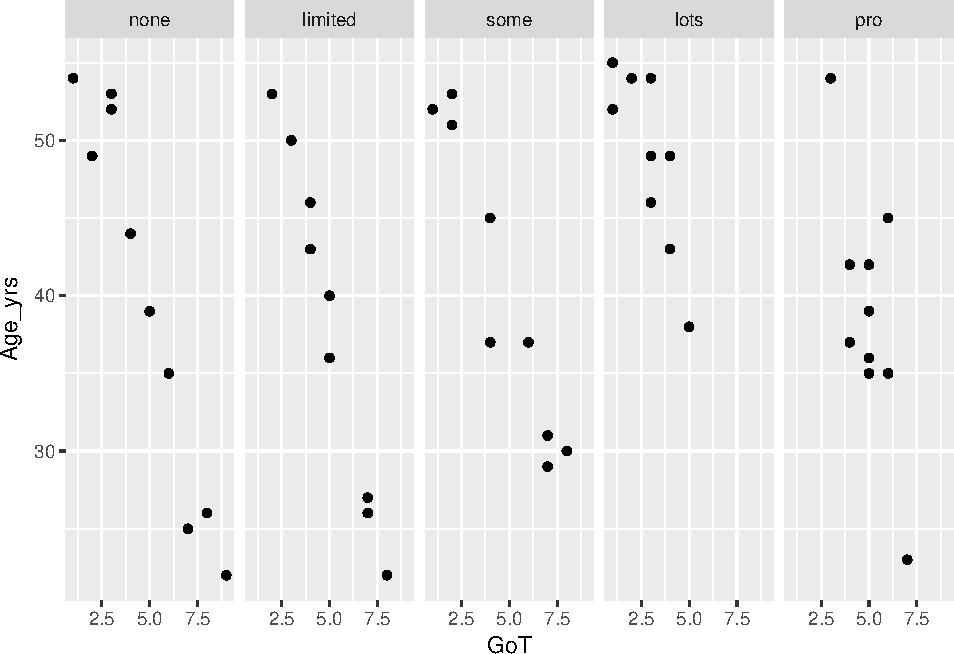
\includegraphics{gilmore-lebreton-hallquist_files/figure-latex/GoT-by-age-exp-1.pdf}
\caption{\label{fig:GoT-by-age-exp}Game of Thrones enthusiasm by age and R
experience}
\end{figure}

\begin{figure}[htbp]
\centering
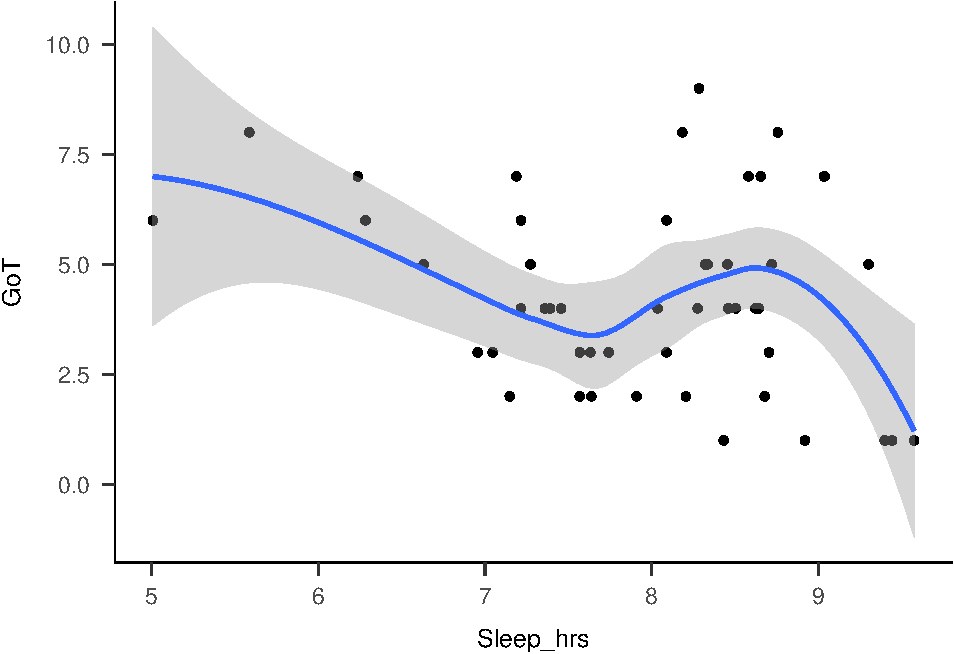
\includegraphics{gilmore-lebreton-hallquist_files/figure-latex/GoT-by-sleep-1.pdf}
\caption{\label{fig:GoT-by-sleep}Game of Thrones enthusiasm by preferred
hours of sleep}
\end{figure}

\begin{table}[tbp]
\begin{center}
\begin{threeparttable}
\caption{\label{tab:GoT-aov-table}ANOVA table for the analyis of the example data set.}
\begin{tabular}{lrcrrrl}
\toprule
Effect & \multicolumn{1}{c}{$F$} & \multicolumn{1}{c}{$\mathit{df}_1$} & \multicolumn{1}{c}{$\mathit{df}_2$} & \multicolumn{1}{c}{$\mathrm{MSE}$} & \multicolumn{1}{c}{$p$} & \multicolumn{1}{c}{$\eta^2_p$}\\
\midrule
R exp & 2.72 & 4 & 40 & 4.19 & .043 & .214\\
Tidy data & 0.00 & 1 & 40 & 4.19 & .985 & .000\\
R exp $\times$ Tidy data & 1.02 & 4 & 40 & 4.19 & .410 & .092\\
\bottomrule
\addlinespace
\end{tabular}
\begin{tablenotes}[para]
\textit{Note.} This is a table created using apa\_print() and apa\_table().
\end{tablenotes}
\end{threeparttable}
\end{center}
\end{table}

Table \ref{tab:GoT-by-experience} summarizes the Game of Thrones ratings
data by levels of R experience.

Let's examine the correlations between our continuous variables. As
indicated in Table \ref{tab:apa-corr-table}, there is a negative
correlation (\(r = -.93\), 95\% CI \([-.96\), \(-.88]\)) between Game of
Thrones enthusiasm and age (\(t(48) = -17.78\), \(p < .001\)), a
negative correlation (\(r = -.25\), 95\% CI \([-.49\), \(.03]\)) between
Game of Thrones enthusiasm and sleep (\(t(48) = -1.78\), \(p = .082\)),
but no correlation (\(r = -.01\), 95\% CI \([-.29\), \(.27]\)) between
age and sleep (\(t(48) = -0.07\), \(p = .944\)). Figures
\ref{fig:GoT-by-age-exp} and \ref{fig:GoT-by-sleep} depict these
patterns.

To test the hypothesis that GoT enthusiasm varies as a function of R
expertise and the extent to which respondents use tidy data, we carried
out a one-way ANOVA. R experience (\(F(4, 40) = 2.72\),
\(\mathrm{MSE} = 4.19\), \(p = .043\), \(\eta^2_p = .214\)) and the use
of tidy data principles (\(F(1, 40) = 0.00\), \(\mathrm{MSE} = 4.19\),
\(p = .985\), \(\eta^2_p = .000\)) did not predict enthusiasm for Game
of Thrones. Table \ref{tab:GoT-aov-table} summarizes these results.

\section{Discussion}\label{discussion}

These results show how awesome it can be to use R, R Markdown, and
literate programming principles to conduct and open, transparent, and
reproducible psychological science. Yay, us!

There are no limitations to what we can accomplish using these tools.
So, let's get to it.

\newpage

\section{References}\label{references}

\setlength{\parindent}{-0.5in} \setlength{\leftskip}{0.5in}

\hypertarget{refs}{}
\hypertarget{ref-R-papaja}{}
Aust, F., \& Barth, M. (2017). \emph{papaja: Create APA manuscripts with
R Markdown}. Retrieved from \url{https://github.com/crsh/papaja}

\hypertarget{ref-R-googlesheets}{}
Bryan, J., \& Zhao, J. (2017). \emph{Googlesheets: Manage google
spreadsheets from r}. Retrieved from
\url{https://CRAN.R-project.org/package=googlesheets}

\hypertarget{ref-R-Hmisc}{}
Harrell Jr, F. E., Charles Dupont, \& others. (2017). \emph{Hmisc:
Harrell miscellaneous}.

\hypertarget{ref-R-purrr}{}
Henry, L., \& Wickham, H. (2017). \emph{Purrr: Functional programming
tools}. Retrieved from \url{https://CRAN.R-project.org/package=purrr}

\hypertarget{ref-R-bindrcpp}{}
Müller, K. (2016). \emph{Bindrcpp: An 'rcpp' interface to active
bindings}. Retrieved from
\url{https://CRAN.R-project.org/package=bindrcpp}

\hypertarget{ref-R-base}{}
R Core Team. (2017). \emph{R: A language and environment for statistical
computing}. Vienna, Austria: R Foundation for Statistical Computing.
Retrieved from \url{https://www.R-project.org/}

\hypertarget{ref-R-lattice}{}
Sarkar, D. (2008). \emph{Lattice: Multivariate data visualization with
r}. New York: Springer. Retrieved from
\url{http://lmdvr.r-forge.r-project.org}

\hypertarget{ref-Simmons2011-za}{}
Simmons, J. P., Nelson, L. D., \& Simonsohn, U. (2011). False-positive
psychology: Undisclosed flexibility in data collection and analysis
allows presenting anything as significant. \emph{Psychol. Sci.},
\emph{22}(11), 1359--1366. Retrieved from
\url{http://journals.sagepub.com/doi/abs/10.1177/0956797611417632}

\hypertarget{ref-R-survival-book}{}
Terry M. Therneau, \& Patricia M. Grambsch. (2000). \emph{Modeling
survival data: Extending the Cox model}. New York: Springer.

\hypertarget{ref-R-ggplot2}{}
Wickham, H. (2009). \emph{Ggplot2: Elegant graphics for data analysis}.
Springer-Verlag New York. Retrieved from \url{http://ggplot2.org}

\hypertarget{ref-R-tidyr}{}
Wickham, H. (2017a). \emph{Tidyr: Easily tidy data with 'spread()' and
'gather()' functions}. Retrieved from
\url{https://CRAN.R-project.org/package=tidyr}

\hypertarget{ref-R-tidyverse}{}
Wickham, H. (2017b). \emph{Tidyverse: Easily install and load
'tidyverse' packages}. Retrieved from
\url{https://CRAN.R-project.org/package=tidyverse}

\hypertarget{ref-R-dplyr}{}
Wickham, H., \& Francois, R. (2016). \emph{Dplyr: A grammar of data
manipulation}. Retrieved from
\url{https://CRAN.R-project.org/package=dplyr}

\hypertarget{ref-R-tibble}{}
Wickham, H., Francois, R., \& Müller, K. (2017). \emph{Tibble: Simple
data frames}. Retrieved from
\url{https://CRAN.R-project.org/package=tibble}

\hypertarget{ref-R-readr}{}
Wickham, H., Hester, J., \& Francois, R. (2017). \emph{Readr: Read
rectangular text data}. Retrieved from
\url{https://CRAN.R-project.org/package=readr}

\hypertarget{ref-R-Formula}{}
Zeileis, A., \& Croissant, Y. (2010). Extended model formulas in R:
Multiple parts and multiple responses. \emph{Journal of Statistical
Software}, \emph{34}(1), 1--13. Retrieved from
\url{http://www.jstatsoft.org/v34/i01/}






\end{document}
